%%%%%%%%%%%%%%%%%%%%%%%%%%%%%%%%%%%%%%%%%%%%%%%%%%%%%%%%%%%%%%%%%%%%%%%%%%%%%%%%%%%%%
%%%%%%%%%%%%%%%%%%%%%%%%%%%%%%%%%%%%%%%%%%%%%%%%%%%%%%%%%%%%%%%%%%%%%%%%%%%%%%%%%%%%%

\setbeamercolor{block title}{bg=white, fg=black}
\setbeamercolor{body}{bg=blue!20}

%%%%%%%%%%%%%%%%%%%%%%%%%%%%%%%%%%%%%%%%%%%%%%%%%%%%%%%%%%%%%%%%%%%%%%%%%%%%%%%%%%%%%%
%%%%%%%%%%%%%%%%%%%%%%%%%%%%%%%%%%%%%%%%%%%%%%%%%%%%%%%%%%%%%%%%%%%%%%%%%%%%%%%%%%%%%%

\begin{frame}
	\frametitle{Problem}
	\begin{itemize}
		\item All compilers contains bugs
		\item Relatively new programming language Kotlin compiler --- not an exclusion
	\end{itemize}
\end{frame}


%%%%%%%%%%%%%%%%%%%%%%%%%%%%%%%%%%%%%%%%%%%%%%%%%%%%%%%%%%%%%%%%%%%%%%%%%%%%%%%%%%%%%%
%%%%%%%%%%%%%%%%%%%%%%%%%%%%%%%%%%%%%%%%%%%%%%%%%%%%%%%%%%%%%%%%%%%%%%%%%%%%%%%%%%%%%%

\begin{frame}
	\frametitle{Main problem in compiler fuzzing}
\setbeamercolor{postit}{bg=red!20}
	\begin{beamercolorbox}[sep=1em]{postit}
		\centering
		How to generate random, non-trivial and semantically valid program to test the compiler?
	\end{beamercolorbox}

\end{frame}


%%%%%%%%%%%%%%%%%%%%%%%%%%%%%%%%%%%%%%%%%%%%%%%%%%%%%%%%%%%%%%%%%%%%%%%%%%%%%%%%%%%%%%
%%%%%%%%%%%%%%%%%%%%%%%%%%%%%%%%%%%%%%%%%%%%%%%%%%%%%%%%%%%%%%%%%%%%%%%%%%%%%%%%%%%%%%

\begin{frame}
	\frametitle{Existing methods}
	\begin{itemize}
		\item Grammar-aware generation ``CSmith'' approaches
			\begin{itemize}
				\item CSmith
				\item YARPGen
				\item jsfunfuzz
				\item ...
			\end{itemize}
	\end{itemize}
\end{frame}

%%%%%%%%%%%%%%%%%%%%%%%%%%%%%%%%%%%%%%%%%%%%%%%%%%%%%%%%%%%%%%%%%%%%%%%%%%%%%%%%%%%%%%
%%%%%%%%%%%%%%%%%%%%%%%%%%%%%%%%%%%%%%%%%%%%%%%%%%%%%%%%%%%%%%%%%%%%%%%%%%%%%%%%%%%%%%

\begin{frame}
	\frametitle{Existing methods}
	\begin{itemize}
		\item Mutation approaches
			\begin{itemize}
				\item jsfunfuzz
				\item ...
				\item skeletal program enumeration
			\end{itemize}
	\end{itemize}
	
\end{frame}

%%%%%%%%%%%%%%%%%%%%%%%%%%%%%%%%%%%%%%%%%%%%%%%%%%%%%%%%%%%%%%%%%%%%%%%%%%%%%%%%%%%%%%
%%%%%%%%%%%%%%%%%%%%%%%%%%%%%%%%%%%%%%%%%%%%%%%%%%%%%%%%%%%%%%%%%%%%%%%%%%%%%%%%%%%%%%

\begin{frame}[fragile]
	\frametitle{Skeletal program enumeration}
\begin{minipage}{0.4\linewidth}
Program P:
		\begin{lstlisting}[language=Kotlin]
var a: Int = 1
var b: Int = 1

while (b < 100) {
    val c = b
    b = a + b
    a = c
}
 \end{lstlisting}
	\end{minipage}
	\begin{minipage}{0.1\linewidth}
	\ \ 
	\end{minipage}
	\begin{minipage}{0.4\linewidth}
Skeleton P':
		\begin{lstlisting}[language=Kotlin]
var [_]: Int = 1
var [_]: Int = 1

while ([_] < 100) {
    val [_] = [_]
    [_] = [_] + [_]
    [_] = [_]
}
	\end{lstlisting}
\end{minipage}
	
\end{frame}


%%%%%%%%%%%%%%%%%%%%%%%%%%%%%%%%%%%%%%%%%%%%%%%%%%%%%%%%%%%%%%%%%%%%%%%%%%%%%%%%%%%%%%
%%%%%%%%%%%%%%%%%%%%%%%%%%%%%%%%%%%%%%%%%%%%%%%%%%%%%%%%%%%%%%%%%%%%%%%%%%%%%%%%%%%%%%

\begin{frame}[fragile]
	\frametitle{Skeletal program enumeration}
\begin{minipage}{0.4\linewidth}
Skeleton P':
		\begin{lstlisting}[language=Kotlin]
var [_]: Int = 1
var [_]: Int = 1

while ([_] < 100) {
    val [_] = [_]
    [_] = [_] + [_]
    [_] = [_]
}
 \end{lstlisting}
	\end{minipage}
	\begin{minipage}{0.1\linewidth}
	\ \ 
	\end{minipage}
	\begin{minipage}{0.4\linewidth}
Produced program P1:
		\begin{lstlisting}[language=Kotlin]
var a: Int = 1
var c: Int = 1

while (a < 100) {
    val b = a
    c = a + c
    a = c
}
	\end{lstlisting}
\end{minipage}
	
\setbeamercolor{postit}{bg=green!20}
	\begin{beamercolorbox}[sep=1em]{postit}
		\centering
		200+ GCC/Clang bugs
	\end{beamercolorbox}
\end{frame}

%%%%%%%%%%%%%%%%%%%%%%%%%%%%%%%%%%%%%%%%%%%%%%%%%%%%%%%%%%%%%%%%%%%%%%%%%%%%%%%%%%%%%%
%%%%%%%%%%%%%%%%%%%%%%%%%%%%%%%%%%%%%%%%%%%%%%%%%%%%%%%%%%%%%%%%%%%%%%%%%%%%%%%%%%%%%%


\begin{frame}[fragile]
	\frametitle{Type-centric fuzzing}
	\begin{itemize}
		\item Inspired by skeletal program enumeration
		\item Placeholders --- expressions
		\item Fill placeholders by compatible typed generated expressions
	\end{itemize}
\ \\ \ \\
\begin{minipage}{0.4\linewidth}
SPE:
\begin{lstlisting}[language=Kotlin]
val a: Int = 1
\end{lstlisting}
 \ \ \ \ \ \ \ \ \ \ \ \ $\downarrow$
\begin{lstlisting}[language=Kotlin]
val [_]: Int = 1
\end{lstlisting}
	\end{minipage}
	\begin{minipage}{0.1\linewidth}
	\ \ 
	\end{minipage}
	\begin{minipage}{0.4\linewidth}
TCE:
\begin{lstlisting}[language=Kotlin]
val a: Int = 1
\end{lstlisting}
 \ \ \ \ \ \ \ \ \ \ \ \ \ \ \ $\downarrow$
\begin{lstlisting}[language=Kotlin]
val a: Int = [Int]
\end{lstlisting}
\end{minipage}
\end{frame}

%%%%%%%%%%%%%%%%%%%%%%%%%%%%%%%%%%%%%%%%%%%%%%%%%%%%%%%%%%%%%%%%%%%%%%%%%%%%%%%%%%%%%%
%%%%%%%%%%%%%%%%%%%%%%%%%%%%%%%%%%%%%%%%%%%%%%%%%%%%%%%%%%%%%%%%%%%%%%%%%%%%%%%%%%%%%%

\begin{frame}[fragile]
	\frametitle{Type centric fuzzing example}
\begin{minipage}{0.4\linewidth}
Program P:
		\begin{lstlisting}[language=Kotlin,basicstyle=\footnotesize]
class A(val a: Int)

fun f(): Int {
    ...
}

var a: Int = 1
var b: Int = 1

while (b < 100) {
    val c = b
    b = a + b
    a = c
}
 \end{lstlisting}
	\end{minipage}
	\begin{minipage}{0.1\linewidth}
	\ \ 
	\end{minipage}
	\begin{minipage}{0.4\linewidth}
Skeleton P':
		\begin{lstlisting}[language=Kotlin,basicstyle=\footnotesize]
class A(val a: Int)

fun f(): Int {
    ...
}

var a: Int = [Int]
var b: Int = [Int]

while ([Int] < [Int]) {
    val c = [Int]
    [Int] = [[Int] + [Int]]
    [Int] = [Int]
}
	\end{lstlisting}
\end{minipage}
	
\end{frame}

%%%%%%%%%%%%%%%%%%%%%%%%%%%%%%%%%%%%%%%%%%%%%%%%%%%%%%%%%%%%%%%%%%%%%%%%%%%%%%%%%%%%%%
%%%%%%%%%%%%%%%%%%%%%%%%%%%%%%%%%%%%%%%%%%%%%%%%%%%%%%%%%%%%%%%%%%%%%%%%%%%%%%%%%%%%%%

\begin{frame}[fragile]
	\frametitle{Type centric fuzzing example}
\begin{minipage}{0.4\linewidth}
Skeleton P':
		\begin{lstlisting}[language=Kotlin,basicstyle=\footnotesize]
class A(val a: Int)

fun f(): Int {
    ...
}

var a: Int = [Int]
var b: Int = [Int]

while ([Int] < [Int]) {
    val c = [Int]
    [Int] = [[Int] + [Int]]
    [Int] = [Int]
}
 \end{lstlisting}
	\end{minipage}
	\begin{minipage}{0.1\linewidth}
	\ \ 
	\end{minipage}
	\begin{minipage}{0.4\linewidth}
Produced program P1:
		\begin{lstlisting}[language=Kotlin,basicstyle=\footnotesize]
class A(val a: Int)

fun f(): Int {
    ...
}

var a: Int = -100
var b: Int = a * f()

while (a < b) {
    val c = 12345
    b = A(f()).a
    b = b
}
	\end{lstlisting}
\end{minipage}
	
\end{frame}

%%%%%%%%%%%%%%%%%%%%%%%%%%%%%%%%%%%%%%%%%%%%%%%%%%%%%%%%%%%%%%%%%%%%%%%%%%%%%%%%%%%%%%
%%%%%%%%%%%%%%%%%%%%%%%%%%%%%%%%%%%%%%%%%%%%%%%%%%%%%%%%%%%%%%%%%%%%%%%%%%%%%%%%%%%%%%

\begin{frame}
	\frametitle{Type-centric fuzzing scheme}
		\begin{itemize}
			\item Generate expressions to fill the placeholders (generation phase)
			\item Fill skeleton by generated expressions (mutation phase)
		\end{itemize}
\end{frame}
%%%%%%%%%%%%%%%%%%%%%%%%%%%%%%%%%%%%%%%%%%%%%%%%%%%%%%%%%%%%%%%%%%%%%%%%%%%%%%%%%%%%%%
%%%%%%%%%%%%%%%%%%%%%%%%%%%%%%%%%%%%%%%%%%%%%%%%%%%%%%%%%%%%%%%%%%%%%%%%%%%%%%%%%%%%%%

\begin{frame}[fragile]
	\frametitle{Generation phase}
	Given:
	\begin{itemize}
		\item Set of variables $V$ 
		\item Available callables $C$
	\end{itemize}
	\ \\ \ \\
			\begin{lstlisting}[language=Kotlin,basicstyle=\footnotesize]
class A(                             //c1
    val a: Int                       //c2
) {                
    fun f(a: String): Int { ... }    //c3
}

val a: Int = 1                       //v1

		\end{lstlisting}
\end{frame}

%%%%%%%%%%%%%%%%%%%%%%%%%%%%%%%%%%%%%%%%%%%%%%%%%%%%%%%%%%%%%%%%%%%%%%%%%%%%%%%%%%%%%%
%%%%%%%%%%%%%%%%%%%%%%%%%%%%%%%%%%%%%%%%%%%%%%%%%%%%%%%%%%%%%%%%%%%%%%%%%%%%%%%%%%%%%%

\begin{frame}[fragile]
	\frametitle{Generation phase}
	We need to generate set of typed expressions using the $C$:
\begin{lstlisting}[language=Kotlin,basicstyle=\footnotesize]
class A(                             //A(1) -> A
    val a: Int                       //A(1).a -> Int
) {                
    fun f(a: String): Int { ... }    //A(1).f("") -> Int
}
\end{lstlisting}
\end{frame}

%%%%%%%%%%%%%%%%%%%%%%%%%%%%%%%%%%%%%%%%%%%%%%%%%%%%%%%%%%%%%%%%%%%%%%%%%%%%%%%%%%%%%%
%%%%%%%%%%%%%%%%%%%%%%%%%%%%%%%%%%%%%%%%%%%%%%%%%%%%%%%%%%%%%%%%%%%%%%%%%%%%%%%%%%%%%%

\begin{frame}[fragile]
\frametitle{Generation phase algorithm}
\newcommand{\adaptTypeParameters}{\text{adaptTypeParams}}%
\newcommand{\args}{\mathit{args}}%
\newcommand{\callee}{\mathit{callee}}%
\newcommand{\call}{\mathit{call}}%
\newcommand{\ffile}{\mathit{file}}%
\newcommand{\findImplementation}{\text{findImplementation}}%
\newcommand{\generateCall}{\text{genCall}}%
\newcommand{\generateClassInstance}{\text{genClassInstance}}%
\newcommand{\generateConstructorCall}{\text{genConstructorCall}}%
\newcommand{\generateConstructor}{\text{genConstructor}}%
\newcommand{\generateInstance}{\text{genInstance}}%
\newcommand{\generateTypeParams}{\text{genTypeParams}}%
\newcommand{\generateValue}{\text{genValue}}%
\newcommand{\getCallables}{\text{getCallables}}%
\newcommand{\getInstanceCallables}{\text{getInstanceCallables}}%
\newcommand{\getRandomConstructor}{\text{getRandomConstructor}}%
\newcommand{\hasOpenConstructor}{\text{hasOpenConstructor}}%
\newcommand{\iCallee}{\mathit{iCallee}}%
\newcommand{\impl}{\mathit{impl}}%
\newcommand{\instance}{\mathit{instance}}%
\newcommand{\is}{\ \mathit{is}\ }%
\newcommand{\klass}{\mathit{class}}%
\newcommand{\parameterize}{\text{parameterize}}%
\newcommand{\randomCtor}{\mathit{randomCtor}}%
\newcommand{\res}{\mathit{res}}%
\newcommand{\typeParams}{\mathit{typeParams}}%
\newcommand{\usages}{\mathit{usages}}%


%%%%%%%%%%%%%%%%%%%%%%%%%%%%%%%%%%%%%%%%%%%%%%%%%%%%%%%%%%%%%%%%%%%%%%%%%%%%%%%
\algdef{SE}[FUNCTION]{Function}{EndFunction}%
   [2]{\algorithmicfunction\ \textproc{#1}\ifthenelse{\equal{#2}{}}{}{(#2)}}%
   {\algorithmicend\ \algorithmicfunction }

\begin{figure}[tb]
\setlength{\leftskip}{0cm}
\small
\textbf{INPUT:} $\ffile$ with a seed program $P$ \\
\textbf{OUTPUT:} list of generated expressions $c_0...c_N$ \\
\begin{algorithmic}[1]


\Function{generationPhase}{$\ffile$}
    \State $\res \leftarrow \left[ \, \right]$
    
    \For{$\callee \in \getCallables(\ffile)$}
        \If{$\callee \is Class$}
            \State $\instance \leftarrow \generateClassInstance(\callee, \ffile)$
            \For{$\iCallee \in \getCallables(\instance)$}
                \State $\res \leftarrow \res + \generateCall(\iCallee, \ffile)$
            \EndFor
        \Else
            \State $\res \leftarrow \res + \generateCall(\callee, \ffile)$
        \EndIf
    \EndFor
    \State \Return $\res$
\EndFunction

%\\
%\Function{genClassInstance}{$\klass, \ffile$}
%    \State $\typeParams \leftarrow \generateTypeParams(\klass, \ffile)$
%    \State $\klass \leftarrow \parameterize(\klass, \typeParams)$
%    \If{$ \neg \hasOpenConstructor(\klass)$}
%        \State $\impl \leftarrow \findImplementation(\klass)$
%        \If{$ \impl \neq null $}
%            \State $\impl \leftarrow \adaptTypeParameters($
%            \State $\qquad \impl, \klass, \typeParams)$
%            \State \Return $\generateClassInstance(\impl, \ffile)$
%        \Else
%            \State \Return $null$
%        \EndIf
%    \EndIf
%    \State $\randomCtor \leftarrow \getRandomConstructor(\klass)$
%    \State \Return $\generateConstructorCall(\randomCtor, \ffile)$
%\EndFunction

% \State $\args \leftarrow \left[ \, \right]$
% \For{$\arg \in \getArgs(\randomCtor)$}
%     \State $\args \leftarrow \args + \generateValue(\arg)$
% \EndFor

\end{algorithmic}
\end{figure}
\end{frame}

\begin{frame}[fragile]
\frametitle{Class instances generation algorithm}
\newcommand{\adaptTypeParameters}{\text{adaptTypeParams}}%
\newcommand{\args}{\mathit{args}}%
\newcommand{\callee}{\mathit{callee}}%
\newcommand{\call}{\mathit{call}}%
\newcommand{\ffile}{\mathit{file}}%
\newcommand{\findImplementation}{\text{findImplementation}}%
\newcommand{\generateCall}{\text{genCall}}%
\newcommand{\generateClassInstance}{\text{genClassInstance}}%
\newcommand{\generateConstructorCall}{\text{genConstructorCall}}%
\newcommand{\generateConstructor}{\text{genConstructor}}%
\newcommand{\generateInstance}{\text{genInstance}}%
\newcommand{\generateTypeParams}{\text{genTypeParams}}%
\newcommand{\generateValue}{\text{genValue}}%
\newcommand{\getCallables}{\text{getCallables}}%
\newcommand{\getInstanceCallables}{\text{getInstanceCallables}}%
\newcommand{\getRandomConstructor}{\text{getRandomConstructor}}%
\newcommand{\hasOpenConstructor}{\text{hasOpenConstructor}}%
\newcommand{\iCallee}{\mathit{iCallee}}%
\newcommand{\impl}{\mathit{impl}}%
\newcommand{\instance}{\mathit{instance}}%
\newcommand{\is}{\ \mathit{is}\ }%
\newcommand{\klass}{\mathit{class}}%
\newcommand{\parameterize}{\text{parameterize}}%
\newcommand{\randomCtor}{\mathit{randomCtor}}%
\newcommand{\res}{\mathit{res}}%
\newcommand{\typeParams}{\mathit{typeParams}}%
\newcommand{\usages}{\mathit{usages}}%


%%%%%%%%%%%%%%%%%%%%%%%%%%%%%%%%%%%%%%%%%%%%%%%%%%%%%%%%%%%%%%%%%%%%%%%%%%%%%%%
\algdef{SE}[FUNCTION]{Function}{EndFunction}%
   [2]{\algorithmicfunction\ \textproc{#1}\ifthenelse{\equal{#2}{}}{}{(#2)}}%
   {\algorithmicend\ \algorithmicfunction }

\begin{figure}[tb]
\setlength{\leftskip}{0cm}
\small

\begin{algorithmic}[1]
\Function{genClassInstance}{$\klass, \ffile$}
    \State $\typeParams \leftarrow \generateTypeParams(\klass, \ffile)$
    \State $\klass \leftarrow \parameterize(\klass, \typeParams)$
    \If{$ \neg \hasOpenConstructor(\klass)$}
        \State $\impl \leftarrow \findImplementation(\klass)$
        \If{$ \impl \neq null $}
            \State $\impl \leftarrow \adaptTypeParameters(\impl, \klass, \typeParams)$
            \State \Return $\generateClassInstance(\impl, \ffile)$
        \Else
            \State \Return $null$
        \EndIf
    \EndIf
    \State $\randomCtor \leftarrow \getRandomConstructor(\klass)$
    \State \Return $\generateConstructorCall(\randomCtor, \ffile)$
\EndFunction

\end{algorithmic}
\end{figure}
\end{frame}


%%%%%%%%%%%%%%%%%%%%%%%%%%%%%%%%%%%%%%%%%%%%%%%%%%%%%%%%%%%%%%%%%%%%%%%%%%%%%%%%%%%%%%
%%%%%%%%%%%%%%%%%%%%%%%%%%%%%%%%%%%%%%%%%%%%%%%%%%%%%%%%%%%%%%%%%%%%%%%%%%%%%%%%%%%%%%

\begin{frame}[fragile]
	\frametitle{Mutation phase}
	Given: 
		\begin{itemize}
			\item Set of generated on previous step expressions $E$
			\item Seed program for mutation phase
		\end{itemize}
	\ \\ \ \\
	\begin{lstlisting}[
  language=Kotlin, basicstyle=\footnotesize
]
// A(1) -> A           | e1
// A(1).a -> Int       | e2
// A(1).f("") -> Int   | e3
// a -> Int            | e4

fun factorial(n: Int): Double {
    var result = 1.0
    for (i in 1..n) {
        result *= i
    }
    return result
}
\end{lstlisting}
\end{frame}

%%%%%%%%%%%%%%%%%%%%%%%%%%%%%%%%%%%%%%%%%%%%%%%%%%%%%%%%%%%%%%%%%%%%%%%%%%%%%%%%%%%%%%
%%%%%%%%%%%%%%%%%%%%%%%%%%%%%%%%%%%%%%%%%%%%%%%%%%%%%%%%%%%%%%%%%%%%%%%%%%%%%%%%%%%%%%

\begin{frame}[fragile]
	\frametitle{Mutation phase}
	Need to make type placeholders and fill it by $e \in E$
	\\ \ \\ \ 
\begin{lstlisting}[
  language=Kotlin, basicstyle=\footnotesize
]
fun factorial(n: Int): Double {
    var result = [Double]
    for (i in [IntRange]) {
        [Double] *= [Int]
    }
    return [Double]
}
\end{lstlisting}
\end{frame}

%%%%%%%%%%%%%%%%%%%%%%%%%%%%%%%%%%%%%%%%%%%%%%%%%%%%%%%%%%%%%%%%%%%%%%%%%%%%%%%%%%%%%%
%%%%%%%%%%%%%%%%%%%%%%%%%%%%%%%%%%%%%%%%%%%%%%%%%%%%%%%%%%%%%%%%%%%%%%%%%%%%%%%%%%%%%%

\begin{frame}[fragile]
	\frametitle{Mutation phase example}
\begin{lstlisting}[
  language=Kotlin, basicstyle=\footnotesize
]
val a: Int = 1

class A(val a: Int) {
    fun f(a: String): Int { ... }
}

fun f(a: Int): Int { ... }

fun factorial(n: Int): Double {
    var result = f(1).toDouble()
    for (i in A(1).f("")..a) {
        result *= i
    }
    return result
}
\end{lstlisting}
\end{frame}

%%%%%%%%%%%%%%%%%%%%%%%%%%%%%%%%%%%%%%%%%%%%%%%%%%%%%%%%%%%%%%%%%%%%%%%%%%%%%%%%%%%%%%
%%%%%%%%%%%%%%%%%%%%%%%%%%%%%%%%%%%%%%%%%%%%%%%%%%%%%%%%%%%%%%%%%%%%%%%%%%%%%%%%%%%%%%

\begin{frame}[fragile]
	\frametitle{How to choose expression to fill?}
	\begin{itemize}
		\item Select a type-compatible expression from $E$
		\item Create a random value of a built-in type~(int, bool, etc.)
		\item Generate a valid call to the standard library
	\end{itemize}
\end{frame}

%%%%%%%%%%%%%%%%%%%%%%%%%%%%%%%%%%%%%%%%%%%%%%%%%%%%%%%%%%%%%%%%%%%%%%%%%%%%%%%%%%%%%%
%%%%%%%%%%%%%%%%%%%%%%%%%%%%%%%%%%%%%%%%%%%%%%%%%%%%%%%%%%%%%%%%%%%%%%%%%%%%%%%%%%%%%%

\begin{frame}[fragile]
	\frametitle{Generation of calls to the standard library}

\begin{lstlisting}[
  language=Kotlin, basicstyle=\footnotesize
]
                // a -> Int  |  [Double] 
\end{lstlisting}
\begin{lstlisting}[
  language=Kotlin, basicstyle=\tiny
]
n = 1:
fun and(other: Int): Int
fun dec(): Int
...
fun toDouble(): Double 
fun minus(other: Double): Double

n = 2:
fun toByte(): Byte
fun times(other: Double): Double

n = 3:
fun toFloat(): Byte
fun compareTo(other: Int): Int
fun plus(other: Double): Double

...

Generated:
a.toDouble()
a.minus(0.0)
a.toByte().times(2.2)
a.toFloat().compareTo(1).plus(0.0)
\end{lstlisting}

\end{frame}

%%%%%%%%%%%%%%%%%%%%%%%%%%%%%%%%%%%%%%%%%%%%%%%%%%%%%%%%%%%%%%%%%%%%%%%%%%%%%%%%%%%%%%
%%%%%%%%%%%%%%%%%%%%%%%%%%%%%%%%%%%%%%%%%%%%%%%%%%%%%%%%%%%%%%%%%%%%%%%%%%%%%%%%%%%%%%

\newcommand{\anon}{\mathit{anon}}%
\newcommand{\anonymize}{\text{anonymize}}%
\newcommand{\eType}{\mathit{eType}}%
\newcommand{\gen}{\mathit{gen}}%
\newcommand{\genPhExpr}{\text{genPhExpr}}%
\newcommand{\genRandomValue}{\text{genRandomValue}}%
\newcommand{\genStdLib}{\text{genStdLib}}%
\newcommand{\getPlaceholders}{\text{getPlaceholders}}%
\newcommand{\getType}{\text{getType}}%
\newcommand{\merge}{\text{merge}}%
\newcommand{\replacePhWithExpr}{\text{replacePhWithExpr}}%
\newcommand{\seed}{\mathit{seed}}%
\newcommand{\type}{\mathit{type}}%

\begin{frame}[fragile]
	\frametitle{Mutation phase algorithm}
\begin{figure}[tb]
\setlength{\leftskip}{0cm}
\textbf{INPUT:} seed program from generation phase $\gen$ \\
\textbf{INPUT:} generated expressions $exprs$ \\
\textbf{INPUT:} seed program for mutation phase $\seed$ \\
\textbf{OUTPUT:} program will filled type placeholders \\
\begin{algorithmic}[1]

\Function{mutationPhase}{}
    \State $\anon \leftarrow \anonymize(\seed)$
    \State $\anon \leftarrow \merge(\anon, \gen)$
    \For{$ph \in \getPlaceholders(\anon)$}
        \State $e \leftarrow \genPhExpr(ph, exprs)$
        \State $\anon \leftarrow \replacePhWithExpr(anon, ph, e)$
    \EndFor
    \State \Return{$\anon$}
\EndFunction
\end{algorithmic}
\end{figure}
\end{frame}

\begin{frame}[fragile]
	\frametitle{Generate phi expression algorithm}
\begin{figure}[tb]
\setlength{\leftskip}{0cm}
\begin{algorithmic}[1]

\Function{genPhExpr}{$ph, exprs$}
    \State $\type \leftarrow \getType(ph)$
    \State $r \leftarrow \left[ \, \right]$
    \State $r \leftarrow r + \genRandomValue(\type)$
    \State $r \leftarrow r + \genStdLib(\type)$
    \For{$e \in exprs$}
        \State $\eType \leftarrow \getType(ph)$
        \If{$compatible(\type, \eType)$}
            \State $r \leftarrow r + e$
        \EndIf
    \EndFor
    \State \Return{$random(r)$}
\EndFunction
\end{algorithmic}
\end{figure}
\end{frame}

%%%%%%%%%%%%%%%%%%%%%%%%%%%%%%%%%%%%%%%%%%%%%%%%%%%%%%%%%%%%%%%%%%%%%%%%%%%%%%%%%%%%%%
%%%%%%%%%%%%%%%%%%%%%%%%%%%%%%%%%%%%%%%%%%%%%%%%%%%%%%%%%%%%%%%%%%%%%%%%%%%%%%%%%%%%%%

\begin{frame}[fragile]
	\frametitle{Mutation phase?}
	Mutation phase can be applied many times:
\center{
\begin{lstlisting}[
  language=Kotlin
]
                    [List<Int>] 
\end{lstlisting}
$\downarrow$
\begin{lstlisting}[
  language=Kotlin
]
                  listOf(1, 2, 3)
\end{lstlisting}
$\downarrow$
\begin{lstlisting}[
  language=Kotlin
]
             listOf([Int], [Int], [Int])
\end{lstlisting}
}
\end{frame}
%%%%%%%%%%%%%%%%%%%%%%%%%%%%%%%%%%%%%%%%%%%%%%%%%%%%%%%%%%%%%%%%%%%%%%%%%%%%%%%%%%%%%%
%%%%%%%%%%%%%%%%%%%%%%%%%%%%%%%%%%%%%%%%%%%%%%%%%%%%%%%%%%%%%%%%%%%%%%%%%%%%%%%%%%%%%%


\begin{frame}
	\frametitle{TCE problems}
	\begin{itemize}
		\item The generation process could potentially never terminate
		\item With iterative TCE run time could increase nonlinearly
		\item Long chains of callables
	\end{itemize}
\end{frame}

%%%%%%%%%%%%%%%%%%%%%%%%%%%%%%%%%%%%%%%%%%%%%%%%%%%%%%%%%%%%%%%%%%%%%%%%%%%%%%%%%%%%%%
%%%%%%%%%%%%%%%%%%%%%%%%%%%%%%%%%%%%%%%%%%%%%%%%%%%%%%%%%%%%%%%%%%%%%%%%%%%%%%%%%%%%%%

\begin{frame}
	\frametitle{Implementation}
We have implemented our approach inside a tool for Kotlin compiler fuzzing named Backend Bug Finder (BBF):
	\begin{figure}
		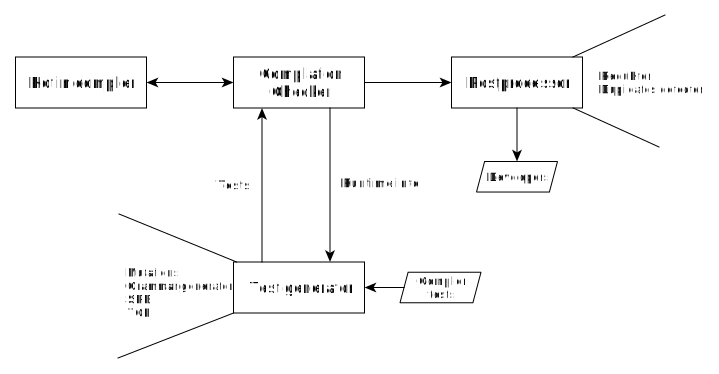
\includegraphics[width=80mm]{image/bbf_scheme}
	\end{figure}	
\end{frame}

%%%%%%%%%%%%%%%%%%%%%%%%%%%%%%%%%%%%%%%%%%%%%%%%%%%%%%%%%%%%%%%%%%%%%%%%%%%%%%%%%%%%%%
%%%%%%%%%%%%%%%%%%%%%%%%%%%%%%%%%%%%%%%%%%%%%%%%%%%%%%%%%%%%%%%%%%%%%%%%%%%%%%%%%%%%%%

\begin{frame}
	\frametitle{Postprocessing}
\end{frame}

%%%%%%%%%%%%%%%%%%%%%%%%%%%%%%%%%%%%%%%%%%%%%%%%%%%%%%%%%%%%%%%%%%%%%%%%%%%%%%%%%%%%%%
%%%%%%%%%%%%%%%%%%%%%%%%%%%%%%%%%%%%%%%%%%%%%%%%%%%%%%%%%%%%%%%%%%%%%%%%%%%%%%%%%%%%%%

\begin{frame}
	\frametitle{Evaluation}
\end{frame}

%%%%%%%%%%%%%%%%%%%%%%%%%%%%%%%%%%%%%%%%%%%%%%%%%%%%%%%%%%%%%%%%%%%%%%%%%%%%%%%%%%%%%%
%%%%%%%%%%%%%%%%%%%%%%%%%%%%%%%%%%%%%%%%%%%%%%%%%%%%%%%%%%%%%%%%%%%%%%%%%%%%%%%%%%%%%%

\begin{frame}
	\frametitle{Interesting bugs found}
\end{frame}

%%%%%%%%%%%%%%%%%%%%%%%%%%%%%%%%%%%%%%%%%%%%%%%%%%%%%%%%%%%%%%%%%%%%%%%%%%%%%%%%%%%%%%
%%%%%%%%%%%%%%%%%%%%%%%%%%%%%%%%%%%%%%%%%%%%%%%%%%%%%%%%%%%%%%%%%%%%%%%%%%%%%%%%%%%%%%

\begin{frame}
	\frametitle{Discussion?}
\end{frame}

%%%%%%%%%%%%%%%%%%%%%%%%%%%%%%%%%%%%%%%%%%%%%%%%%%%%%%%%%%%%%%%%%%%%%%%%%%%%%%%%%%%%%%
%%%%%%%%%%%%%%%%%%%%%%%%%%%%%%%%%%%%%%%%%%%%%%%%%%%%%%%%%%%%%%%%%%%%%%%%%%%%%%%%%%%%%%

\begin{frame}
	\frametitle{Conclusion}
\end{frame}

%%%%%%%%%%%%%%%%%%%%%%%%%%%%%%%%%%%%%%%%%%%%%%%%%%%%%%%%%%%%%%%%%%%%%%%%%%%%%%%%%%%%%%%
%%%%%%%%%%%%%%%%%%%%%%%%%%%%%%%%%%%%%%%%%%%%%%%%%%%%%%%%%%%%%%%%%%%%%%%%%%%%%%%%%%%%%%%
%\begin{frame}[fragile]
%	\frametitle{Example of posted Kotlin compiler bug}
%	\tiny{
%	\begin{lstlisting}[language = Kotlin]
%open class A1(y: String) {
%    val x = "[A1.x,$y]"
%}
%open class A2(y: String) {
%    val x = "[A2.x,$y]"
%    inner open class B1 : A1 {
%        constructor(p: String) : super("[B1.param,$p]")
%        fun foo() = x + ";" + this@A2.x + ";"
%    }
%    fun bar(): String {
%        return with(A2("#bar")) {
%            class C : B1("bar") {}
%            C().foo()
%        }
%    }
%    fun foo() = A2("#baz").baz()
%    fun A2.baz(): String {
%        class C : B1("baz") {}
%        return C().foo()
%    }
%}
%fun box(): String {
%    val r3 = A2("f").bar()
%    if (r3 != "[A1.x,[B1.param,bar]];[A2.x,#bar];") return "$r3:"
%    val r4 = A2("gg").foo()
%    if (r4 != "[A1.x,[B1.param,baz]];[A2.x,#baz];") return "$r:"
%    return "OK"
%}
%	\end{lstlisting}
%	}
%\end{frame}
%
%%%%%%%%%%%%%%%%%%%%%%%%%%%%%%%%%%%%%%%%%%%%%%%%%%%%%%%%%%%%%%%%%%%%%%%%%%%%%%%%%%%%%%%
%%%%%%%%%%%%%%%%%%%%%%%%%%%%%%%%%%%%%%%%%%%%%%%%%%%%%%%%%%%%%%%%%%%%%%%%%%%%%%%%%%%%%%%
%
%\begin{frame}
%	\frametitle{Existing methods}
%	\begin{itemize}
%		\item Language-agnostic methods
%			\begin{itemize}
%				\item Delta-debugging
%				\item Slicing
%				\item Hierarchical delta-debugging
%				\item Generalized tree reduction
%				\item Perses
%				\item Pardis
%			\end{itemize}
%	\end{itemize}		
%	
%\end{frame}
%
%%%%%%%%%%%%%%%%%%%%%%%%%%%%%%%%%%%%%%%%%%%%%%%%%%%%%%%%%%%%%%%%%%%%%%%%%%%%%%%%%%%%%%%
%%%%%%%%%%%%%%%%%%%%%%%%%%%%%%%%%%%%%%%%%%%%%%%%%%%%%%%%%%%%%%%%%%%%%%%%%%%%%%%%%%%%%%%
%
%\begin{frame}[fragile]
%	\frametitle{Result of language-agnostic method application}
%	\tiny{
%	\begin{lstlisting}[language = Kotlin]
%open class A1(y: String)
%class A2(y: String) {
%    val x = "[A2.x,$y]"
%
%    inner open class B1 : A1 {
%        constructor(p: String) : super("[B1.param,$p]")
%
%        fun foo() = x + ";" + this@A2.x + ";"
%    }
%
%    fun A2.baz(): String {
%        class C : B1("baz")
%        return C().foo()
%    }
%}
%	\end{lstlisting}
%	}
%\end{frame}
%
%
%%%%%%%%%%%%%%%%%%%%%%%%%%%%%%%%%%%%%%%%%%%%%%%%%%%%%%%%%%%%%%%%%%%%%%%%%%%%%%%%%%%%%%%
%%%%%%%%%%%%%%%%%%%%%%%%%%%%%%%%%%%%%%%%%%%%%%%%%%%%%%%%%%%%%%%%%%%%%%%%%%%%%%%%%%%%%%%
%
%\begin{frame}[fragile]
%	\frametitle{Minimal reproducing sample}
%	\begin{lstlisting}[language = Kotlin]
%open class A1
%
%class A2 {
%    open inner class B1 : A1()
%    
%    fun A2.baz() {
%        class C : B1()
%    }
%}
%	\end{lstlisting}
%\end{frame}
%
%%%%%%%%%%%%%%%%%%%%%%%%%%%%%%%%%%%%%%%%%%%%%%%%%%%%%%%%%%%%%%%%%%%%%%%%%%%%%%%%%%%%%%%
%%%%%%%%%%%%%%%%%%%%%%%%%%%%%%%%%%%%%%%%%%%%%%%%%%%%%%%%%%%%%%%%%%%%%%%%%%%%%%%%%%%%%%%
%
%\begin{frame}
%	\frametitle{Existing methods}
%	\begin{itemize}
%		\item Language-agnostic methods
%			\begin{itemize}
%				\item[•] Delta-debugging
%				\item[•] Slicing
%				\item[•] Hierarchical delta-debugging
%				\item[•] Generalized tree reduction
%				\item[•] Perses
%				\item[•] Pardis
%			\end{itemize}
%		\item Language-specific methods
%			\begin{itemize}
%				\item Text-based
%				\item Tree-based
%			\end{itemize}
%		\item Combination of language-agnostic and language-specific methods
%			\begin{itemize}
%				\item C-Reduce
%			\end{itemize}
%	\end{itemize}		
%	
%\end{frame}
%
%
%%%%%%%%%%%%%%%%%%%%%%%%%%%%%%%%%%%%%%%%%%%%%%%%%%%%%%%%%%%%%%%%%%%%%%%%%%%%%%%%%%%%%%%
%%%%%%%%%%%%%%%%%%%%%%%%%%%%%%%%%%%%%%%%%%%%%%%%%%%%%%%%%%%%%%%%%%%%%%%%%%%%%%%%%%%%%%%
%
%\begin{frame}
%	\frametitle{C-Reduce}
%		\begin{itemize}
%				\item C language reduktor
%				\item Set of source code plugins 
%				\begin{itemize}
%					\item Delta-debugging
%					\item Source code transformations
%					\item Result formatting
%				\end{itemize}
%				\item Shows better results than level-agnostic methods but have performance problems
%		\end{itemize}
%\end{frame}
%
%%%%%%%%%%%%%%%%%%%%%%%%%%%%%%%%%%%%%%%%%%%%%%%%%%%%%%%%%%%%%%%%%%%%%%%%%%%%%%%%%%%%%%%
%%%%%%%%%%%%%%%%%%%%%%%%%%%%%%%%%%%%%%%%%%%%%%%%%%%%%%%%%%%%%%%%%%%%%%%%%%%%%%%%%%%%%%%
%
%\begin{frame}[fragile]
%	\frametitle{Approach}
%	\begin{itemize}
%		\item So we decided to combine language-agnostic techniques and language-specific transformations
%		\item Our approach looks as follows:
%	\end{itemize}
%	\begin{figure}
%		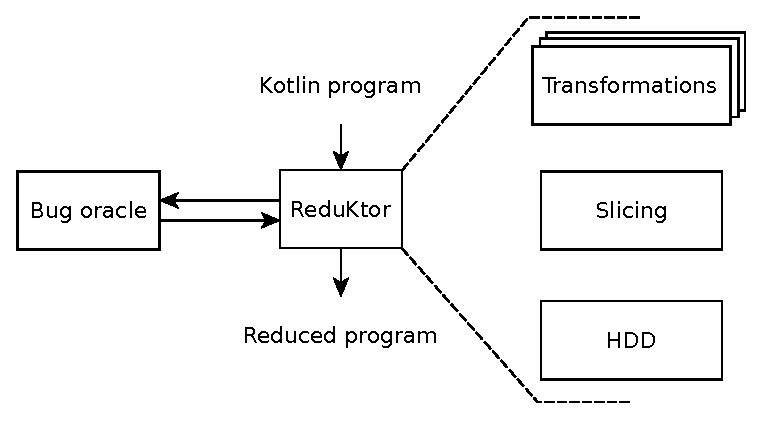
\includegraphics[width=80mm]{image/overviewNew}
%	\end{figure}	
%
%\end{frame}
%
%%%%%%%%%%%%%%%%%%%%%%%%%%%%%%%%%%%%%%%%%%%%%%%%%%%%%%%%%%%%%%%%%%%%%%%%%%%%%%%%%%%%%%%
%%%%%%%%%%%%%%%%%%%%%%%%%%%%%%%%%%%%%%%%%%%%%%%%%%%%%%%%%%%%%%%%%%%%%%%%%%%%%%%%%%%%%%%
%
%\begin{frame}[fragile]
%	\frametitle{Oracle}
%	\begin{itemize}
%		\item If $P$ fails on $T$, it should fail on $T'$ with same error
%		\item We are checking it by comparing of error messages
%	\end{itemize}
%	\begin{figure}[tb]
%	\tiny{
%\begin{lstlisting}[style=kotlin]
%@Error:Kotlin: [Internal Error] kotlin.codegen.CompilationException: 
%Back-end (JVM) Internal error: wrong code generated
%kotlin.codegen.CompilationException Back-end (JVM) Internal error:@
%Couldn't transform method node:
%test ()V:
%   L0
%    LINENUMBER 2 L0
%   L1
%    POP
%   L2
%...
%Cause: AFTER mandatory stack transformations: incorrect bytecode
%Element is unknown The root cause was thrown at: MethodVerifier.kt:28
%File being compiled at position: @(10,1)@ in Main.kt
%...
%\end{lstlisting}
%}
%\end{figure}
%\end{frame}
%
%%%%%%%%%%%%%%%%%%%%%%%%%%%%%%%%%%%%%%%%%%%%%%%%%%%%%%%%%%%%%%%%%%%%%%%%%%%%%%%%%%%%%%%
%%%%%%%%%%%%%%%%%%%%%%%%%%%%%%%%%%%%%%%%%%%%%%%%%%%%%%%%%%%%%%%%%%%%%%%%%%%%%%%%%%%%%%%
%
%\begin{frame}
%	\frametitle{Transformations}
%	We implemented transformations over two types of representation:
%		\begin{itemize}
%			\item Textual
%			\item Syntax tree
%		\end{itemize}
%\end{frame}
%%%%%%%%%%%%%%%%%%%%%%%%%%%%%%%%%%%%%%%%%%%%%%%%%%%%%%%%%%%%%%%%%%%%%%%%%%%%%%%%%%%%%%%
%%%%%%%%%%%%%%%%%%%%%%%%%%%%%%%%%%%%%%%%%%%%%%%%%%%%%%%%%%%%%%%%%%%%%%%%%%%%%%%%%%%%%%%
%
%\begin{frame}
%	\frametitle{Text transformations}
%	\begin{itemize}
%		\item We selected about 30 of various text transformations to be used based on the following:
%			\begin{itemize}
%    				\item Our Kotlin programming experience
%    				\item Transformations used in other reduction tools
%    				\item Transformations used in the Kotlin IntelliJ IDEA plugin for code simplification
%			\end{itemize}
%	\end{itemize}
%\end{frame}
%
%%%%%%%%%%%%%%%%%%%%%%%%%%%%%%%%%%%%%%%%%%%%%%%%%%%%%%%%%%%%%%%%%%%%%%%%%%%%%%%%%%%%%%%
%%%%%%%%%%%%%%%%%%%%%%%%%%%%%%%%%%%%%%%%%%%%%%%%%%%%%%%%%%%%%%%%%%%%%%%%%%%%%%%%%%%%%%%
%
%\begin{frame}[fragile]
%	\frametitle{Text transformations example}
%\begin{minipage}{0.4\linewidth}
%	Before:
%		\begin{lstlisting}[style=crs_cpp]
%fun f() {
%    var a = 124125125
%    val b = a + 1
%    val c = 1.1
%    var d: Double
%    while (a.toDouble() != c) {
%        d = a * b * c
%        a += 1
%    }
%    println("a = $a")
%}
% \end{lstlisting}
%	\end{minipage}
%	\begin{minipage}{0.1\linewidth}
%	\ \ 
%	\end{minipage}
%	\begin{minipage}{0.4\linewidth}
%	After:
%		\begin{lstlisting}[style=crs_cpp]
%fun f() {
%    var a = 0
%    val b = a + 1
%    val c = 0.0
%    var d: Double
%    if (a.toDouble() != c) {
%        d = a * b
%        a++
%    }
%    println("")
%}
% \end{lstlisting}
%	\end{minipage}
%\end{frame}
%
%
%%%%%%%%%%%%%%%%%%%%%%%%%%%%%%%%%%%%%%%%%%%%%%%%%%%%%%%%%%%%%%%%%%%%%%%%%%%%%%%%%%%%%%%
%%%%%%%%%%%%%%%%%%%%%%%%%%%%%%%%%%%%%%%%%%%%%%%%%%%%%%%%%%%%%%%%%%%%%%%%%%%%%%%%%%%%%%%
%
%\begin{frame}
%	\frametitle{Syntax tree based transformations}
%	\begin{itemize}
%	\item More than 30 transformations
%	\item Can be divided on the next groups:
%	\begin{itemize}
%    		\item Expression simplification
%    		\item Removal of unneeded components
%    		\item Simplification of interdependencies
%    		\item Others
%	\end{itemize}
%	\end{itemize}
%\end{frame}
%
%%%%%%%%%%%%%%%%%%%%%%%%%%%%%%%%%%%%%%%%%%%%%%%%%%%%%%%%%%%%%%%%%%%%%%%%%%%%%%%%%%%%%%%
%%%%%%%%%%%%%%%%%%%%%%%%%%%%%%%%%%%%%%%%%%%%%%%%%%%%%%%%%%%%%%%%%%%%%%%%%%%%%%%%%%%%%%%
%
%\begin{frame}[fragile]
%	\frametitle{Syntax tree based transformations example}
%		\begin{lstlisting}[style=Kotlin]
%fun f(a: Int): @@String@@ {
%    val answer = when (a) {
%        1 -> "1"
%        2 -> "2"
%        @3 -> "4"@
%        else -> ""
%    }
%    @@return answer@@
%}
% \end{lstlisting}
%
%\end{frame}
%
%%%%%%%%%%%%%%%%%%%%%%%%%%%%%%%%%%%%%%%%%%%%%%%%%%%%%%%%%%%%%%%%%%%%%%%%%%%%%%%%%%%%%%%
%%%%%%%%%%%%%%%%%%%%%%%%%%%%%%%%%%%%%%%%%%%%%%%%%%%%%%%%%%%%%%%%%%%%%%%%%%%%%%%%%%%%%%%
%
%\begin{frame}[fragile]
%	\frametitle{Syntax tree based transformations example}
%		\begin{lstlisting}[style=Kotlin]
%fun f(a: Int) {
%    @@val answer =@@ when (a) {
%        1 -> "1"
%        2 -> "2"
%        3 -> "4"
%        else -> ""
%    }
%}
% \end{lstlisting}
%
%\end{frame}
%
%%%%%%%%%%%%%%%%%%%%%%%%%%%%%%%%%%%%%%%%%%%%%%%%%%%%%%%%%%%%%%%%%%%%%%%%%%%%%%%%%%%%%%%
%%%%%%%%%%%%%%%%%%%%%%%%%%%%%%%%%%%%%%%%%%%%%%%%%%%%%%%%%%%%%%%%%%%%%%%%%%%%%%%%%%%%%%%
%
%\begin{frame}[fragile]
%	\frametitle{Syntax tree based transformations example}
%		\begin{lstlisting}[style=Kotlin]
%fun f(a: Int) {
%    when (a) {
%        @@1 -> "1"
%        2 -> "2"@@
%        3 -> "4"
%        else -> ""
%    }
%}
% \end{lstlisting}
%
%\end{frame}
%
%%%%%%%%%%%%%%%%%%%%%%%%%%%%%%%%%%%%%%%%%%%%%%%%%%%%%%%%%%%%%%%%%%%%%%%%%%%%%%%%%%%%%%%
%%%%%%%%%%%%%%%%%%%%%%%%%%%%%%%%%%%%%%%%%%%%%%%%%%%%%%%%%%%%%%%%%%%%%%%%%%%%%%%%%%%%%%%
%
%\begin{frame}[fragile]
%	\frametitle{Syntax tree based transformations example}
%		\begin{lstlisting}[style=Kotlin]
%fun f(@@a: Int@@) {
%    when (@@a@@) {
%        3 -> "4"
%        else -> ""
%    }
%}
% \end{lstlisting}
%
%\end{frame}
%
%%%%%%%%%%%%%%%%%%%%%%%%%%%%%%%%%%%%%%%%%%%%%%%%%%%%%%%%%%%%%%%%%%%%%%%%%%%%%%%%%%%%%%%
%%%%%%%%%%%%%%%%%%%%%%%%%%%%%%%%%%%%%%%%%%%%%%%%%%%%%%%%%%%%%%%%%%%%%%%%%%%%%%%%%%%%%%%
%
%\begin{frame}[fragile]
%	\frametitle{Syntax tree based transformations example}
%		\begin{lstlisting}[style=Kotlin]
%fun f() {
%    when (1) {
%        3 -> "4"
%        else -> ""
%    }
%}
% \end{lstlisting}
%
%\end{frame}
%
%
%%%%%%%%%%%%%%%%%%%%%%%%%%%%%%%%%%%%%%%%%%%%%%%%%%%%%%%%%%%%%%%%%%%%%%%%%%%%%%%%%%%%%%%
%%%%%%%%%%%%%%%%%%%%%%%%%%%%%%%%%%%%%%%%%%%%%%%%%%%%%%%%%%%%%%%%%%%%%%%%%%%%%%%%%%%%%%%
%
%\begin{frame}
%	\begin{itemize}
%		\frametitle{Slicing}
%		\item Slicing creates a program slice, free of unneeded parts w.r.t. slicing criterion
%		\item For our purposes we decided to implement a static backward slicing over the syntax trees on the following levels:
%		\begin{itemize}
%			\item Intraprocedural level
%			\item Function level
%			\item Class level
%		\end{itemize}
%	\end{itemize}
%\end{frame}
%
%%%%%%%%%%%%%%%%%%%%%%%%%%%%%%%%%%%%%%%%%%%%%%%%%%%%%%%%%%%%%%%%%%%%%%%%%%%%%%%%%%%%%%%
%%%%%%%%%%%%%%%%%%%%%%%%%%%%%%%%%%%%%%%%%%%%%%%%%%%%%%%%%%%%%%%%%%%%%%%%%%%%%%%%%%%%%%%
%
%\begin{frame}[fragile]
%	\frametitle{Slicing example}
%		\tiny
%	\begin{lstlisting}[style=kotlin]
%class Square(private val a: Double) {
%
%    fun getPerimeter(): Double = a * 4
%
%    fun getSquare(): Double = a * a
%}
%
%
%class Triangle(private val a: Double, private val b: Double, 
%               private val c: Double) {
%
%    fun getPerimeter(): Double = a + b + c
%
%    fun getSquare(): Double {
%        var square = 0.0
%        if (a * a + b * b == c * c) {
%            @square = a * b / 2@
%        } else {
%            val p = getPerimeter() / 2
%            square = Math.sqrt(p * (p - a) * (p - b) * (p - c))
%        }
%        return square
%    }
%
%}
%\end{lstlisting}
%\end{frame}
%
%%%%%%%%%%%%%%%%%%%%%%%%%%%%%%%%%%%%%%%%%%%%%%%%%%%%%%%%%%%%%%%%%%%%%%%%%%%%%%%%%%%%%%%
%%%%%%%%%%%%%%%%%%%%%%%%%%%%%%%%%%%%%%%%%%%%%%%%%%%%%%%%%%%%%%%%%%%%%%%%%%%%%%%%%%%%%%%
%
%\begin{frame}[fragile]
%	\frametitle{Slicing result}
%	\tiny
%	\begin{lstlisting}[style=kotlin]
%class Triangle(private val a: Double, private val b: Double, 
%               private val c: Double) {
%
%    fun getSquare(): Double {
%        var square = 0.0
%        if (a * a + b * b == c * c) {
%            @square = a * b / 2@
%        } else { }
%        return square
%    }
%
%}
%\end{lstlisting}
%\end{frame}
%
%%%%%%%%%%%%%%%%%%%%%%%%%%%%%%%%%%%%%%%%%%%%%%%%%%%%%%%%%%%%%%%%%%%%%%%%%%%%%%%%%%%%%%%
%%%%%%%%%%%%%%%%%%%%%%%%%%%%%%%%%%%%%%%%%%%%%%%%%%%%%%%%%%%%%%%%%%%%%%%%%%%%%%%%%%%%%%%
%
%\begin{frame}[fragile]
%	\frametitle{Hierarchical delta debugging}
%	\begin{itemize}
%	\item Delta-debugging over syntax tree
%	\item Suppose that we have next sample:
%	\end{itemize}
%	\tiny
%		\begin{lstlisting}[style=kotlin]
%fun f() {
%    val a = 1
%    var b = 0
%    
%    if (a != 0) b += 1
%    else b += 2
%    
%    while (b != 0) @- - b@
%}
%\end{lstlisting}
%\end{frame}
%
%%%%%%%%%%%%%%%%%%%%%%%%%%%%%%%%%%%%%%%%%%%%%%%%%%%%%%%%%%%%%%%%%%%%%%%%%%%%%%%%%%%%%%%
%%%%%%%%%%%%%%%%%%%%%%%%%%%%%%%%%%%%%%%%%%%%%%%%%%%%%%%%%%%%%%%%%%%%%%%%%%%%%%%%%%%%%%%
%
%\begin{frame}
%	\frametitle{Hierarchical delta debugging example}
%	\begin{figure}
%		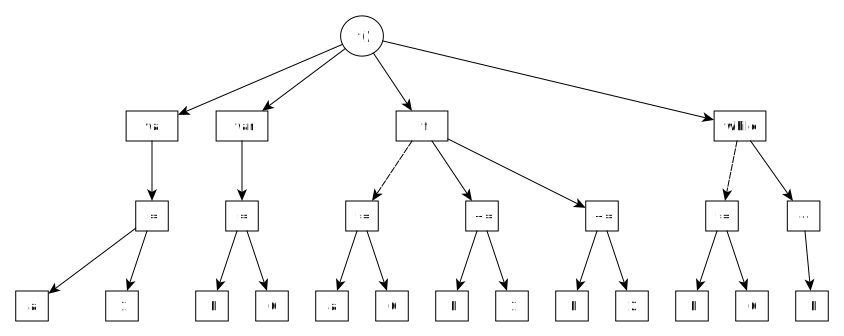
\includegraphics[height=42mm]{image/hdd1}
%	\end{figure}	
%\end{frame}
%
%%%%%%%%%%%%%%%%%%%%%%%%%%%%%%%%%%%%%%%%%%%%%%%%%%%%%%%%%%%%%%%%%%%%%%%%%%%%%%%%%%%%%%%
%%%%%%%%%%%%%%%%%%%%%%%%%%%%%%%%%%%%%%%%%%%%%%%%%%%%%%%%%%%%%%%%%%%%%%%%%%%%%%%%%%%%%%%
%
%\begin{frame}
%	\frametitle{Hierarchical delta debugging example}
%	\begin{figure}
%		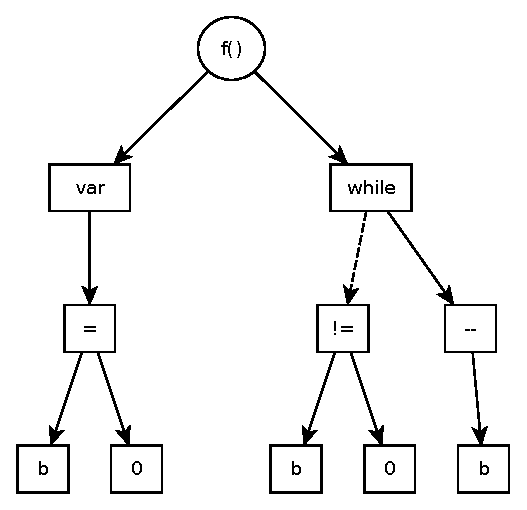
\includegraphics[height=50mm]{image/hdd2}
%	\end{figure}	
%\end{frame}
%
%%%%%%%%%%%%%%%%%%%%%%%%%%%%%%%%%%%%%%%%%%%%%%%%%%%%%%%%%%%%%%%%%%%%%%%%%%%%%%%%%%%%%%%
%%%%%%%%%%%%%%%%%%%%%%%%%%%%%%%%%%%%%%%%%%%%%%%%%%%%%%%%%%%%%%%%%%%%%%%%%%%%%%%%%%%%%%%
%
%\begin{frame}
%	\frametitle{Project level simplification}
%	\begin{itemize}
%		\item We need to support reduction of the projects
%		\item First we have to remove project dependencies
%		\item In Kotlin dependencies of a file are defined via import lists or fully qualified names
%		\item These elements form the dependency tree, which may be used to guide the simplification process
%	\end{itemize}
%\end{frame}
%
%%%%%%%%%%%%%%%%%%%%%%%%%%%%%%%%%%%%%%%%%%%%%%%%%%%%%%%%%%%%%%%%%%%%%%%%%%%%%%%%%%%%%%%
%%%%%%%%%%%%%%%%%%%%%%%%%%%%%%%%%%%%%%%%%%%%%%%%%%%%%%%%%%%%%%%%%%%%%%%%%%%%%%%%%%%%%%%
%
%\begin{frame}[fragile]
%	\frametitle{Project dependencies example} 
%	\begin{figure}
%		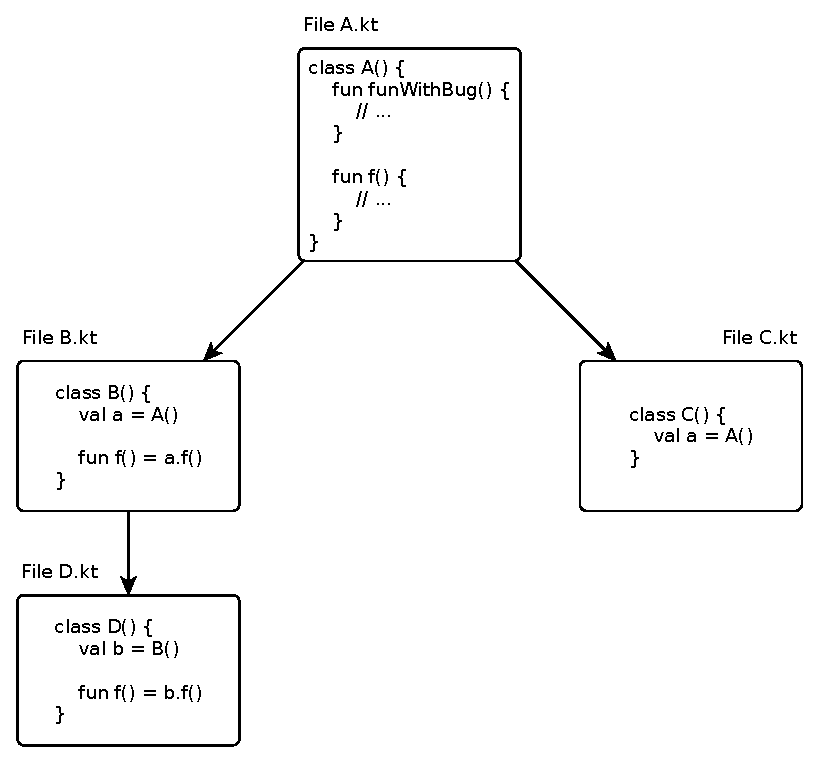
\includegraphics[height=80mm]{image/depTreeExample}
%	\end{figure}	
%\end{frame}
%
%
%%%%%%%%%%%%%%%%%%%%%%%%%%%%%%%%%%%%%%%%%%%%%%%%%%%%%%%%%%%%%%%%%%%%%%%%%%%%%%%%%%%%%%%
%%%%%%%%%%%%%%%%%%%%%%%%%%%%%%%%%%%%%%%%%%%%%%%%%%%%%%%%%%%%%%%%%%%%%%%%%%%%%%%%%%%%%%%
%
%\begin{frame}
%	\frametitle{Transformation order}
%	\begin{itemize}
%		\item Final result may be affected by the order
%		\item Overall performance also depends on the transformation order
%		\item We decided to apply transformations in the order of their “reductiveness”
%	\end{itemize}
%	\begin{figure}
%		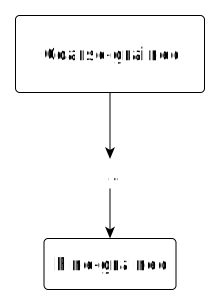
\includegraphics[width=30mm]{image/order}
%	\end{figure}	
%\end{frame}
%
%
%%%%%%%%%%%%%%%%%%%%%%%%%%%%%%%%%%%%%%%%%%%%%%%%%%%%%%%%%%%%%%%%%%%%%%%%%%%%%%%%%%%%%%%
%%%%%%%%%%%%%%%%%%%%%%%%%%%%%%%%%%%%%%%%%%%%%%%%%%%%%%%%%%%%%%%%%%%%%%%%%%%%%%%%%%%%%%%
%
%\begin{frame}
%	\frametitle{Resulting pipeline}
%	The resulting pipeline is as follows:
%	\begin{itemize}
%		\item Project-level simplifications
%		\item Slicing
%		\item Text based transformations
%		\item Syntax tree based transformations
%		\item Hierarchical delta debugging
%	\end{itemize}
%	Every transformation is applied in order until convergence, i.e., until its input stops decreasing in size.
%\end{frame}
%
%%%%%%%%%%%%
%%%%%%%%%%%%
%
%\begin{frame}
%	\frametitle{Implementation}
%	We implemented a prototype tool based on our approach
%%	\begin{figure}
%%		\includegraphics[width=30mm]{image/Reduktor}
%%	\end{figure}	
%	\begin{itemize}
%		\item We decided to use Kotlin compiler like a library
%		\item Parallel processing of independent files
%		\item Caching
%	\end{itemize}
%\end{frame}
%
%%%%%%%%%%%%%%%%%%%%%%%%%%%%%%%%%%%%%%%%%%%%%%%%%%%%%%%%%%%%%%%%%%%%%%%%%%%%%%%%%%%%%%%
%%%%%%%%%%%%%%%%%%%%%%%%%%%%%%%%%%%%%%%%%%%%%%%%%%%%%%%%%%%%%%%%%%%%%%%%%%%%%%%%%%%%%%%
%
%
%\begin{frame}
%	\frametitle{Evaluation}
%	For the evaluation, we run ReduKtor for Kotlin compiler version 1.3.10 on two types of input:
%	\begin{itemize}
%		\item Results of Kotlin compiler fuzzer + data from bug tracker
%		\item Number of real-world projects were injected with invalid code
%	\end{itemize}
%	\begin{figure}
%		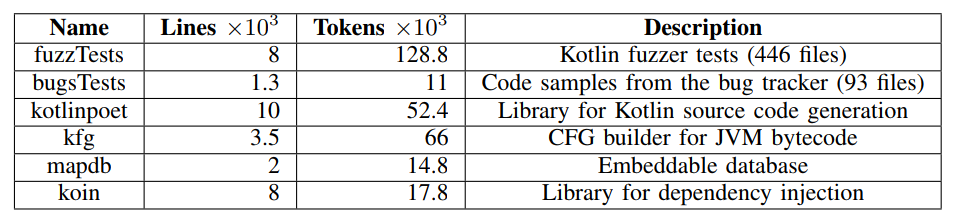
\includegraphics[width=100mm]{image/table1}
%	\end{figure}	
%\end{frame}
%
%%%%%%%%%%%%%%%%%%%%%%%%%%%%%%%%%%%%%%%%%%%%%%%%%%%%%%%%%%%%%%%%%%%%%%%%%%%%%%%%%%%%%%%
%%%%%%%%%%%%%%%%%%%%%%%%%%%%%%%%%%%%%%%%%%%%%%%%%%%%%%%%%%%%%%%%%%%%%%%%%%%%%%%%%%%%%%%
%
%\begin{frame}
%	\frametitle{Evaluation}
%	\begin{figure}
%		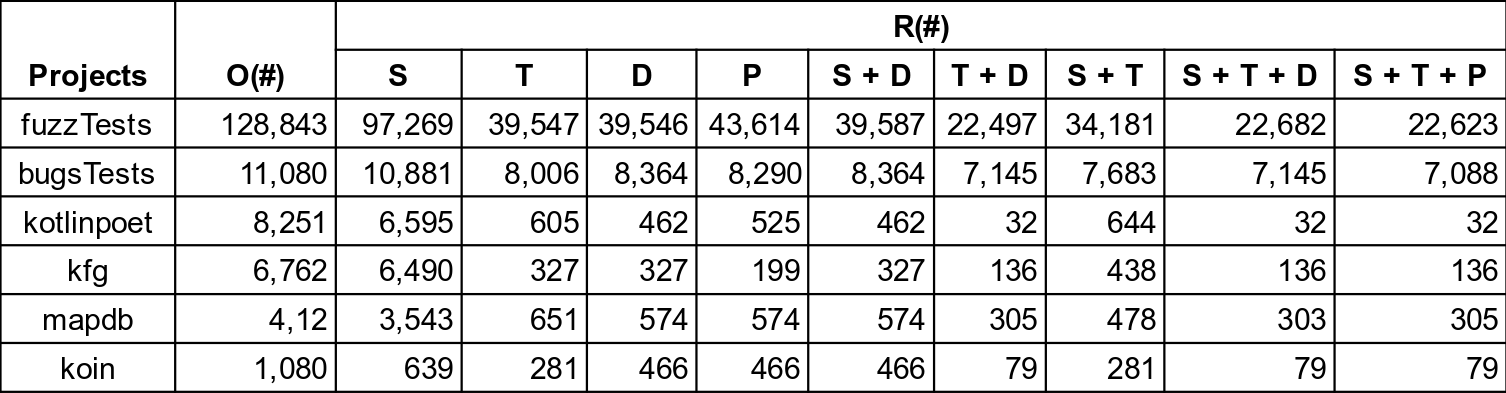
\includegraphics[width=110mm]{image/ev1}
%	\end{figure}	
%	\begin{figure}
%		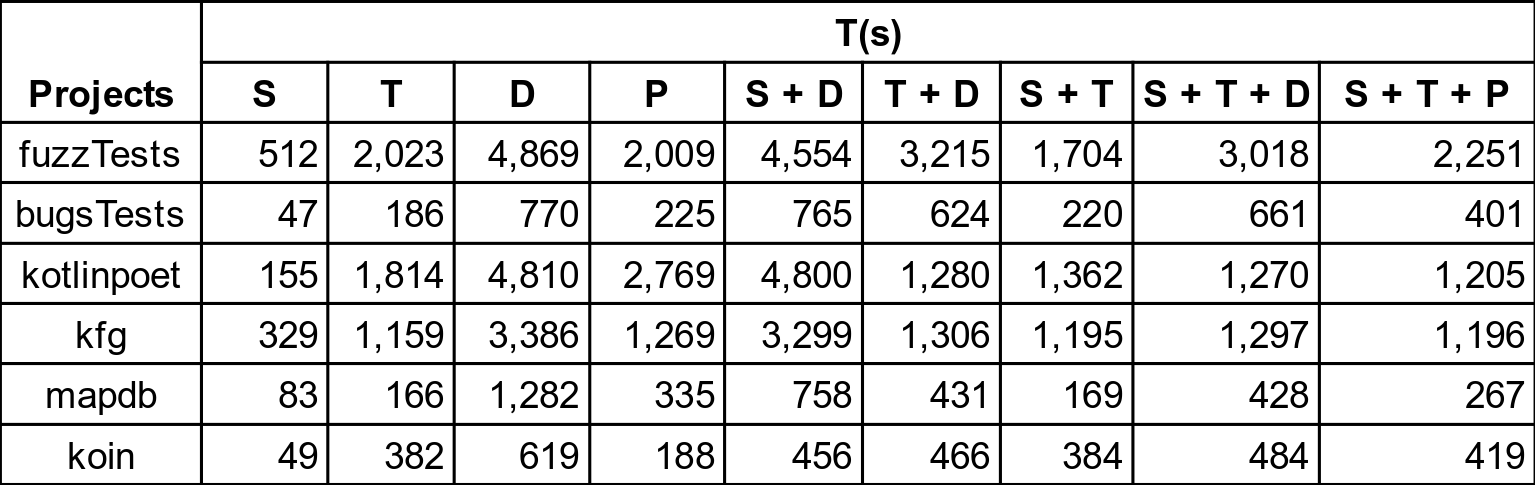
\includegraphics[width=100mm]{image/ev2}
%	\end{figure}	
%\end{frame}
%
%
%%%%%%%%%%%%%%%%%%%%%%%%%%%%%%%%%%%%%%%%%%%%%%%%%%%%%%%%%%%%%%%%%%%%%%%%%%%%%%%%%%%%%%%
%%%%%%%%%%%%%%%%%%%%%%%%%%%%%%%%%%%%%%%%%%%%%%%%%%%%%%%%%%%%%%%%%%%%%%%%%%%%%%%%%%%%%%%
%
%%\begin{frame}
%%	\frametitle{Lessons learned}
%%	\begin{itemize}
%%		\item Slicing impact on the input reduction is negligible
%%		\item Language-specific transformations outperform the language-agnostic techniques
%%		\item The results of language-specific transformations can be improved by applying language-agnostic techniques to their results
%%	\end{itemize}
%%\end{frame}
%
%%%%%%%%%%%%%%%%%%%%%%%%%%%%%%%%%%%%%%%%%%%%%%%%%%%%%%%%%%%%%%%%%%%%%%%%%%%%%%%%%%%%%%%
%%%%%%%%%%%%%%%%%%%%%%%%%%%%%%%%%%%%%%%%%%%%%%%%%%%%%%%%%%%%%%%%%%%%%%%%%%%%%%%%%%%%%%%
%
%\begin{frame}
%	\frametitle{Lessons learned}
%	Slicing impact on the input reduction is negligible
%	\begin{figure}
%		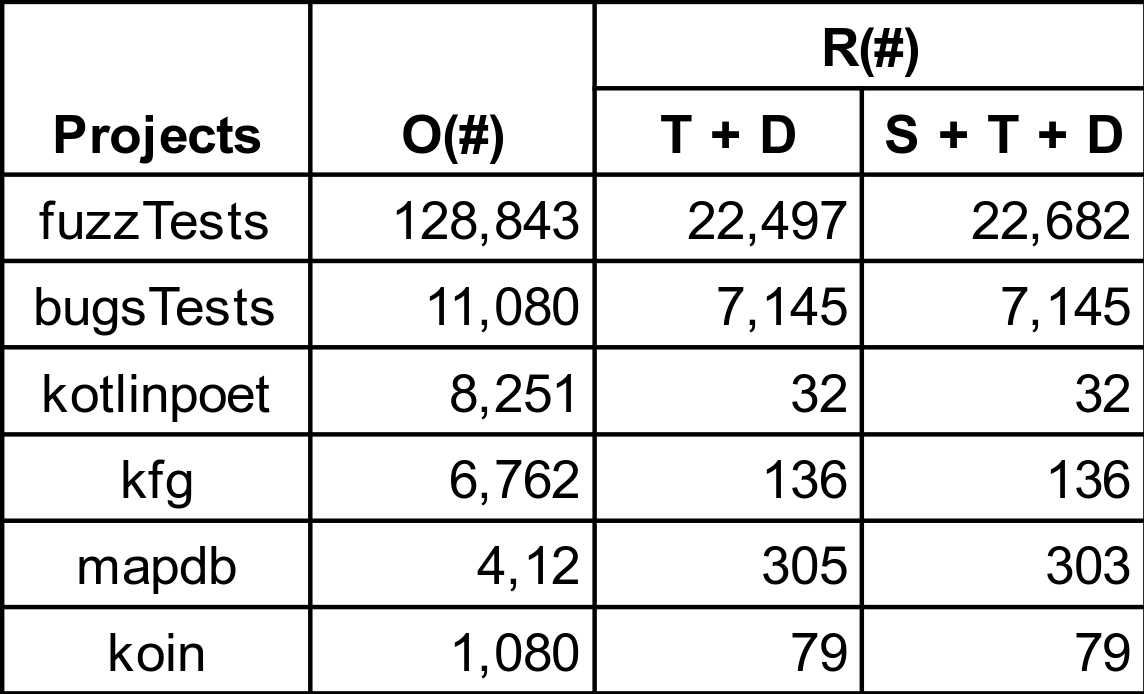
\includegraphics[width=50mm]{image/ev3}
%	\end{figure}	
%		\begin{figure}
%		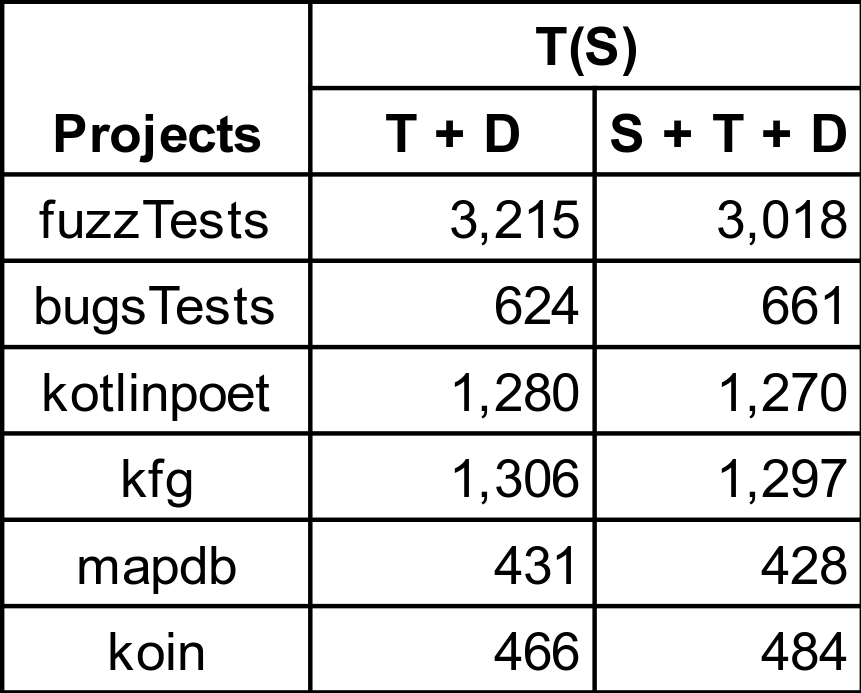
\includegraphics[width=40mm]{image/ev4}
%	\end{figure}	
%\end{frame}
%
%
%%%%%%%%%%%%%%%%%%%%%%%%%%%%%%%%%%%%%%%%%%%%%%%%%%%%%%%%%%%%%%%%%%%%%%%%%%%%%%%%%%%%%%%
%%%%%%%%%%%%%%%%%%%%%%%%%%%%%%%%%%%%%%%%%%%%%%%%%%%%%%%%%%%%%%%%%%%%%%%%%%%%%%%%%%%%%%%
%
%\begin{frame}
%	\frametitle{Lessons learned}
%	Language-specific transformations outperform the language-agnostic techniques
%	\begin{figure}
%		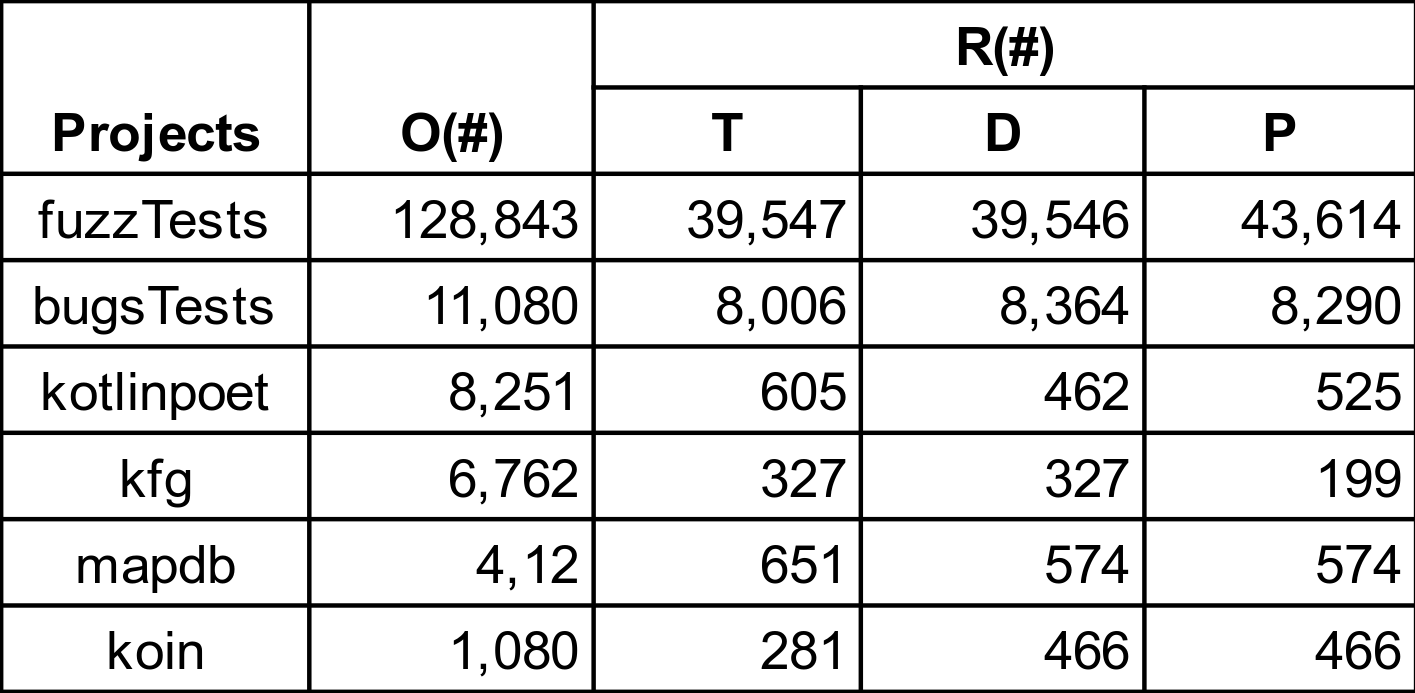
\includegraphics[width=60mm]{image/ev5}
%	\end{figure}	
%		\begin{figure}
%		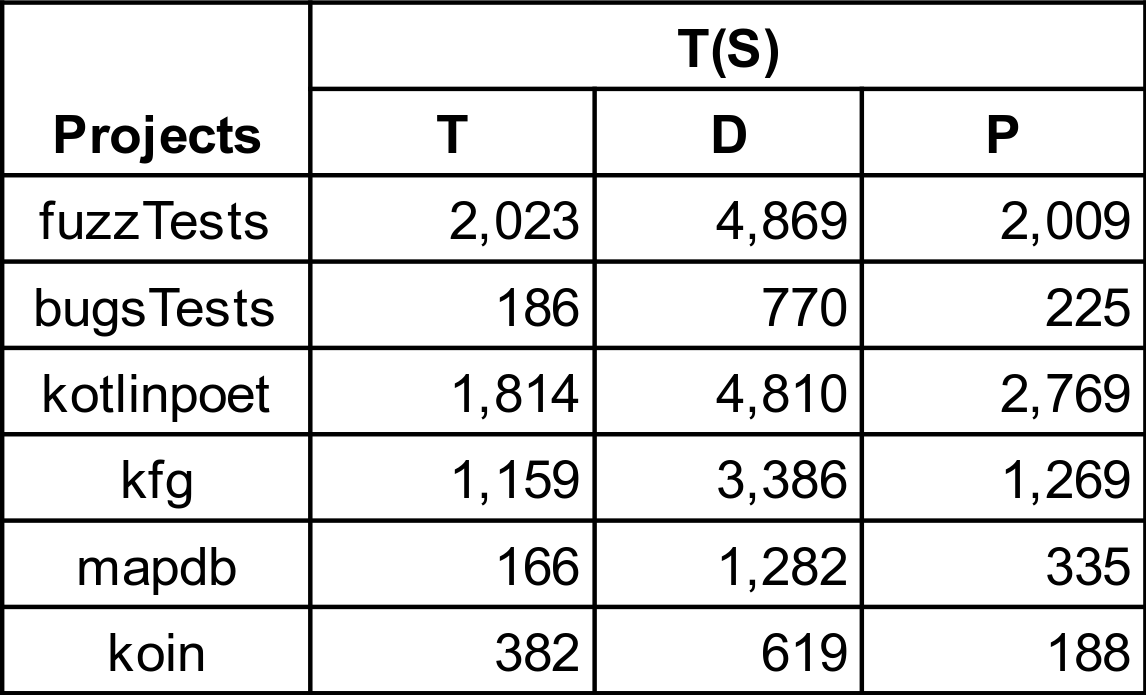
\includegraphics[width=50mm]{image/ev6}
%	\end{figure}	
%\end{frame}
%
%%%%%%%%%%%%%%%%%%%%%%%%%%%%%%%%%%%%%%%%%%%%%%%%%%%%%%%%%%%%%%%%%%%%%%%%%%%%%%%%%%%%%%%
%%%%%%%%%%%%%%%%%%%%%%%%%%%%%%%%%%%%%%%%%%%%%%%%%%%%%%%%%%%%%%%%%%%%%%%%%%%%%%%%%%%%%%%
%
%\begin{frame}
%	\frametitle{Lessons learned}
%	The results of language-specific transformations can be improved by applying language-agnostic techniques to their results
%	\begin{figure}
%		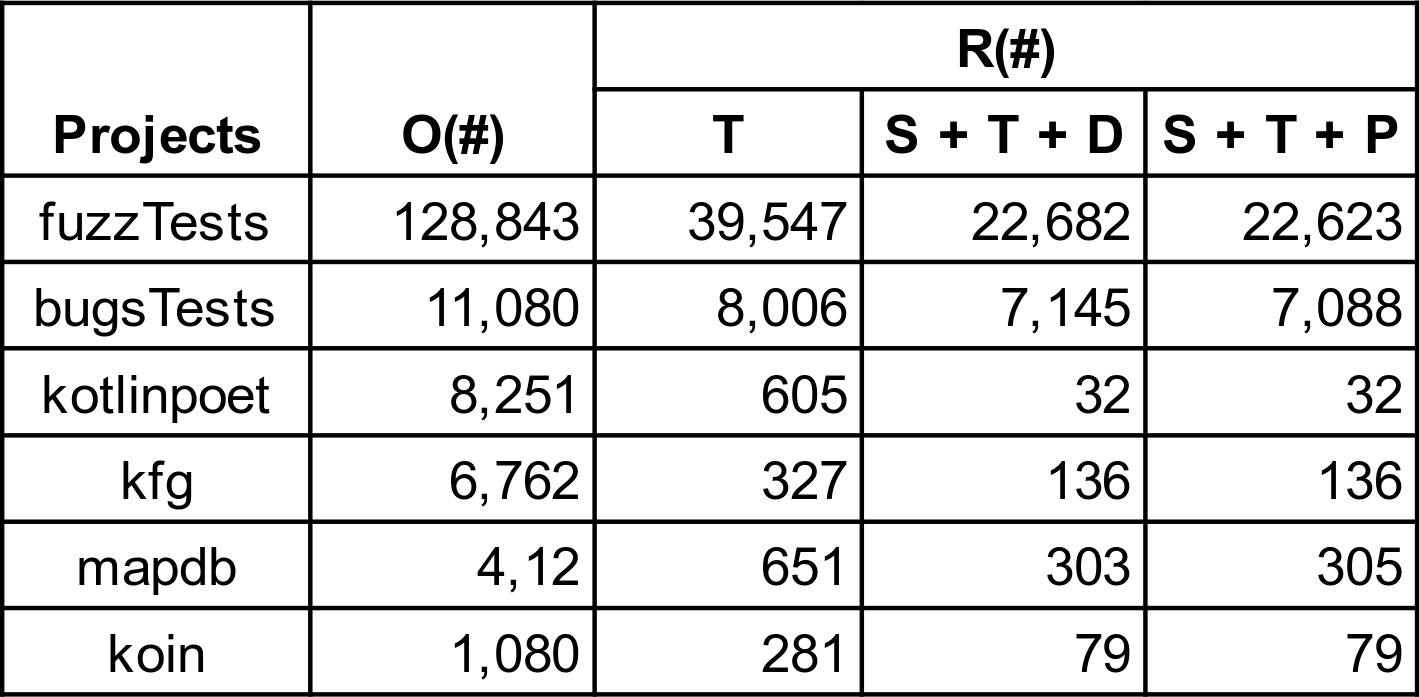
\includegraphics[width=60mm]{image/ev7}
%	\end{figure}	
%		\begin{figure}
%		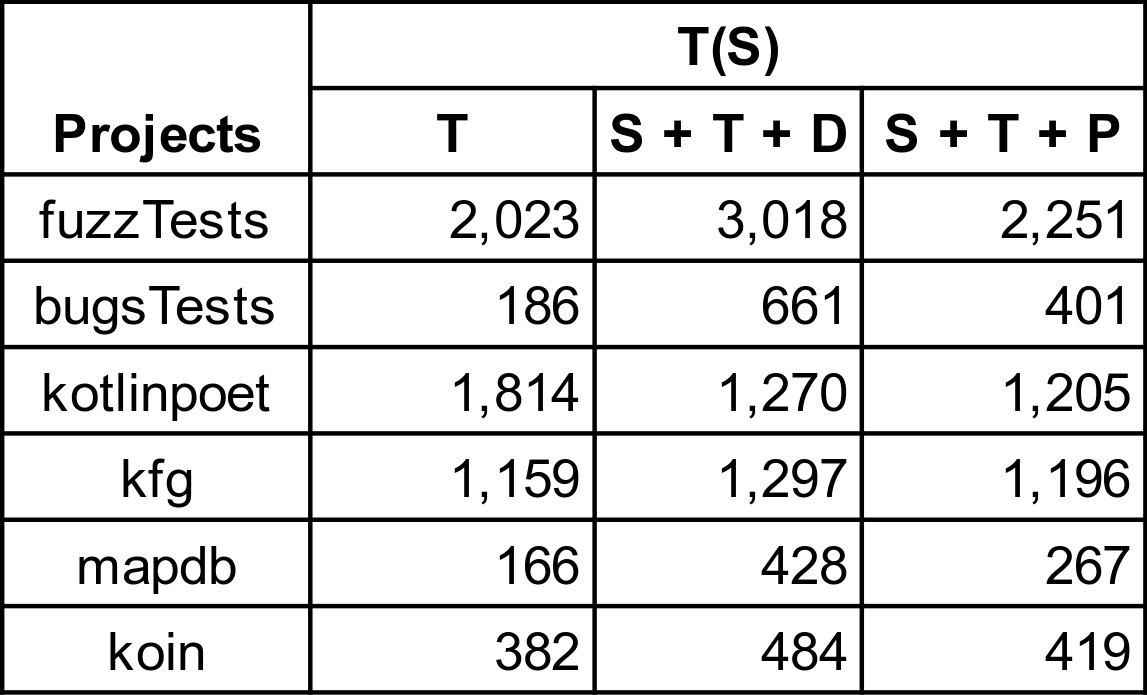
\includegraphics[width=50mm]{image/ev8}
%	\end{figure}	
%\end{frame}
%
%%%%%%%%%%%%%%%%%%%%%%%%%%%%%%%%%%%%%%%%%%%%%%%%%%%%%%%%%%%%%%%%%%%%%%%%%%%%%%%%%%%%%%%
%%%%%%%%%%%%%%%%%%%%%%%%%%%%%%%%%%%%%%%%%%%%%%%%%%%%%%%%%%%%%%%%%%%%%%%%%%%%%%%%%%%%%%%
%
%\begin{frame}
%	\frametitle{Conclusion}
%	4 pictures???
%%	\begin{itemize}
%%		\item We present an approach to automatic input reduction for the Kotlin
%%		\item Implemented a tool called ReduKtor and applied it for some samples
%%		\item 
%%		\item We have already started to collaborate with the Kotlin team
%%	\end{itemize}
%\end{frame}
%
%
%%%%%%%%%%%%%%%%%%%%%%%%%%%%%%%%%%%%%%%%%%%%%%%%%%%%%%%%%%%%%%%%%%%%%%%%%%%%%%%%%%%%%%
%%%%%%%%%%%%%%%%%%%%%%%%%%%%%%%%%%%%%%%%%%%%%%%%%%%%%%%%%%%%%%%%%%%%%%%%%%%%%%%%%%%%%%

\begin{frame}[fragile]
\frametitle{Contact information}
\texttt{\{stepanov, akhin, belyaev\}@kspt.icc.spbstu.ru} \\ \ \\ \ \\
\begin{columns} 
\column{0.33\textwidth} 
	\begin{figure}
		
\includegraphics[width=0.99\linewidth]{image/polytech_logo_en} 
	\end{figure}
\column{0.33\textwidth} 
	\begin{figure}
		
\includegraphics[width=0.99\linewidth]{image/jetbrainsLogo} 
	\end{figure}
\end{columns}
	\begin{figure}
		\includegraphics[width=0.4\linewidth]{image/Reduktor} 
	\end{figure}
\end{frame}